\chapter{Business Model Canvas}

O Business Model Canvas, proposto por Osterwalder e Pigneur (2010), é uma ferramenta utilizada para representar, de forma visual e estruturada, os principais elementos que compõem um modelo de negócio. Por meio de seus blocos, torna-se possível organizar informações essenciais, como proposta de valor, público-alvo, fontes de receita, recursos, atividades e parceiros-chave, favorecendo uma visão mais ampla e integrada do empreendimento.

Nesse sentido, com o objetivo de compreender melhor a lógica de funcionamento do negócio proposto e a relação entre suas dimensões estratégicas e operacionais, foi elaborado o Business Model Canvas apresentado na Figura \ref{fig:canvas}, com base no conceito do produto, nas características do público-alvo e nas definições construídas ao longo do projeto.

\begin{figure}[H]
    \centering
    \caption{Business Model Canvas}
    \label{fig:canvas}
    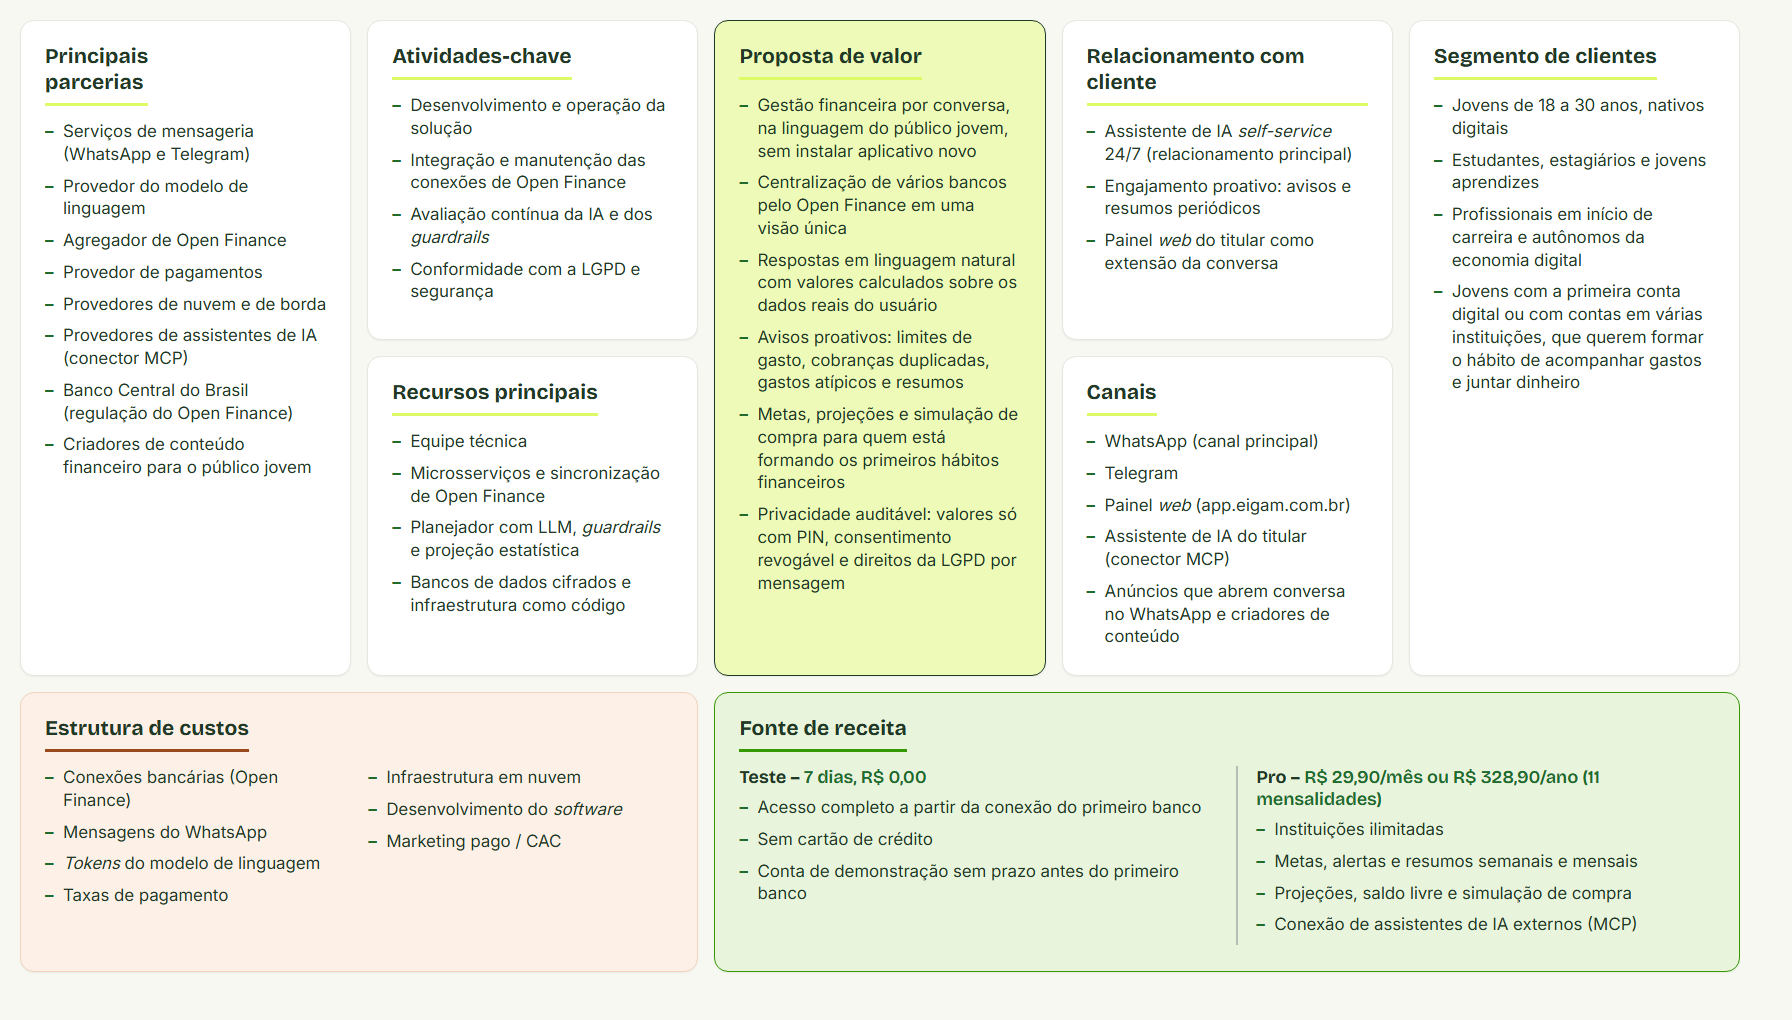
\includegraphics[width=1\textwidth]{images/canvas.png}
    \sourcenote{\textbf{Fonte:} Elaborado pelos autores (\workYear), com base no modelo de Osterwalder e Pigneur (2010).}
\end{figure}

A leitura da Figura~\ref{fig:canvas} mostra a coerência entre os blocos. A proposta de valor, centrada na gestão financeira por conversa, na visão consolidada de vários bancos e na privacidade auditável, responde ao segmento de jovens de 18 a 30 anos que abrem a primeira conta digital ou mantêm contas em várias instituições e chega a ele pela conversa nos mensageiros que esse público já usa, com o WhatsApp como canal principal e o Telegram como segundo canal; essa conversa é complementada pelo painel \textit{web} e pelo assistente de IA do próprio titular. As atividades e os recursos principais concentram-se nos microsserviços, na integração com o Open Finance e na avaliação contínua da IA, com o apoio de parceiros como o agregador de Open Finance, os serviços de mensageria e o provedor do modelo de linguagem. Como os principais custos, que são as conexões bancárias, as mensagens e os \textit{tokens} do modelo de linguagem, crescem com o uso, o acesso aos próprios dados sem assinatura limita-se a um período de teste de sete dias, e a fonte de receita é a assinatura do plano Pro, que reúne os recursos de maior custo de processamento.
